\documentclass[conference]{IEEEtran}
\IEEEoverridecommandlockouts
\usepackage[utf8]{inputenc}
\usepackage[T1]{fontenc}
\usepackage{amsmath,amssymb}
\usepackage{graphicx}
\usepackage{booktabs}
\usepackage{cite}
\usepackage{url}
\usepackage[hidelinks]{hyperref}

\begin{document}

\title{Elo-Based Adaptive Gamification for Programming Practice:\\
Model, Simulation Study and Experimental Protocol}

\author{\IEEEauthorblockN{Danila Zakharov}
\IEEEauthorblockA{\textit{Satbayev University}\\
Almaty, Kazakhstan}}

\maketitle

\begin{abstract}
Gamification is widely used in programming courses, yet its effects are small and inconsistent, and rewards and task order are usually the same for every student. We propose an adaptive gamification model in which an Elo rating estimates student ability and task difficulty, the next task is chosen so that the predicted probability of success is close to 0.7, and experience points depend on difficulty. The model is implemented as a FastAPI service backed by Redis and evaluated on 1,500 simulated students. Adaptive selection kept tasks within the zone of attainable difficulty (success probability 0.5--0.85) in 79\% of attempts versus 40\% for the linear order typical of static gamification; for the weakest third of students the share of successful attempts rose from 0.45 to 0.64. On randomly assigned tasks, the Elo rating predicted success better than static difficulty labels (AUC 0.81 vs.\ 0.78). We also identify a cold-start problem for strong students and show that initialising ability from a pre-test largely removes it. The service handles about 1,700 events per second with a p95 latency of 53~ms. We describe a preregistered three-condition controlled experiment; code and data are open.
\end{abstract}

\begin{IEEEkeywords}
gamification, adaptive learning, Elo rating, programming education, automated assessment, simulation
\end{IEEEkeywords}

\section{Introduction}
Automated assessment systems have become a standard tool for programming practice: a student submits a solution and learns within seconds whether it passes the tests~\cite{wasik2018}. Such systems, however, do not decide \emph{which} task a student should attempt next. In a typical course every student follows the same sequence, so a strong student spends time on trivial exercises while a weak one gets stuck on a task that is still out of reach.

To keep students practising, courses add game elements such as experience points, levels, badges and leaderboards~\cite{deterding2011,denny2013,marin2019}. A meta-analysis by Sailer and Homner~\cite{sailer2020} found a positive but small effect of gamification on learning, with behavioural and motivational effects that are unstable under rigorous designs; some studies even report a decline in intrinsic motivation~\cite{hanus2015}. One possible explanation is that reward rules are identical for all students and ignore how hard a task is \emph{for this student}: the reward for an easy task loses its value, and the reward for an impossible one becomes unattainable.

Adaptive systems have long matched difficulty to the learner. The Elo rating estimates student ability and item difficulty from a stream of attempts without prior calibration~\cite{pelanek2016,klinkenberg2011}. These systems, however, mostly target short-answer items and are not connected to a game layer. We found no model that jointly estimates ability, selects a code-writing task and scales the reward by its difficulty.

This paper proposes such a model and addresses three questions. \textbf{RQ1:} Does adaptive selection keep tasks within the zone of attainable difficulty more often than the linear order of static gamification? \textbf{RQ2:} Which students benefit most, and where does the model fail? \textbf{RQ3:} Does the Elo rating predict success more accurately than static difficulty labels?

Our contributions are: (1)~an adaptive gamification model linking the Elo rating, task selection with a target success probability of 0.7, and experience points; (2)~a simulation study on 1,500 synthetic students showing that adaptive selection keeps tasks in the attainable zone in 79\% of attempts versus 40\% for the linear order, and revealing a cold-start problem for strong students; (3)~an open implementation~\cite{nirm2026code} and a protocol for a three-condition controlled experiment.

\section{Related Work}
\textit{Gamification in education.} Reviews agree that most studies use points, badges and leaderboards and report mostly positive but context-dependent effects~\cite{hamari2014,dicheva2015}. Experimental work links specific elements to need satisfaction~\cite{sailer2017}, while negative effects such as loss of interest and undesired competition are also documented~\cite{toda2018}.

\textit{Gamification in programming courses.} Virtual achievements increased the volume of voluntary practice in an online drill system~\cite{denny2013}; gamified activities improved engagement of computer science students~\cite{ibanez2014}; and a controlled study in programming courses found better results in the gamified group~\cite{marin2019}. In all of these, rewards follow fixed rules.

\textit{Adaptivity.} Pelánek~\cite{pelanek2016} reviews Elo-based estimation in educational systems and proposes an uncertainty function that makes the update step decrease with the number of attempts. Math Garden~\cite{klinkenberg2011} uses a related model to keep the expected success rate near a chosen target. Our work transfers this idea to code-writing tasks and couples it with the reward system.

\section{Model and Simulation Setup}
\subsection{Ability, difficulty and task selection}
The predicted probability that student $s$ with ability $\theta_s$ solves task $q$ with difficulty $d_q$ is
\begin{equation}
P(\theta_s, d_q) = \frac{1}{1 + e^{-(\theta_s - d_q)}}.
\label{eq:p}
\end{equation}
After an attempt with outcome $y \in \{0, 1\}$ both estimates are updated:
\begin{equation}
\theta_s \leftarrow \theta_s + K\,(y - P), \qquad d_q \leftarrow d_q - K_d\,(y - P),
\label{eq:elo}
\end{equation}
with $K = 0.2$ and $K_d = 0.1$ chosen by simulation (Section~\ref{sec:results}). The next task minimises the distance to the target probability $p^{*} = 0.7$:
\begin{equation}
q^{*} = \arg\min_q \left| P(\theta_s, d_q) - p^{*} \right|.
\label{eq:select}
\end{equation}

\subsection{Rewards}
Experience points for a solved task are
$\mathrm{XP} = B\,\delta_q\,\rho^{a-1}\,(1 + \beta \min(\mathit{streak}, 10))$, where $B = 100$, $\delta_q = \max(0.5,\, 1 + d_q/2)$ scales the reward by difficulty, $\rho = 0.85$ penalises each extra attempt $a$, and $\beta = 0.05$ rewards daily streaks. Level thresholds grow geometrically with ratio 1.5, and badges are predicates over the student profile.

\subsection{Simulation}
We simulate 300 students with true ability $\theta^{*} \sim \mathcal{N}(0, 1)$ and 50 tasks with true difficulty evenly spaced on $[-2.5, 2.4]$. Each student makes 60 attempts; outcomes are drawn from (\ref{eq:p}) using true values, while the system sees only outcomes and starts from $\hat\theta = \hat d = 0$. Three policies are compared: \emph{linear} (tasks sorted by a teacher's integer difficulty label; the student advances after a success and repeats the task after a failure), \emph{adaptive} (\ref{eq:select}), and \emph{mixed} (adaptive, but 10\% of tasks are assigned at random). Each configuration is run with five seeds. The main metric is the share of attempts whose true success probability lies in $[0.5, 0.85]$, which we call the zone of attainable difficulty. We report means with 95\% confidence intervals and effect sizes; with simulated data, $p$-values are reported only for completeness.

\section{Results}
\label{sec:results}
\textit{RQ1.} Adaptive selection kept tasks in the attainable zone in 0.79 (95\% CI 0.77--0.81) of attempts versus 0.40 (0.40--0.41) for the linear order; Cohen's $d = 2.8$ (Table~\ref{tab:policies}). The share of successful attempts was 0.71 and 0.58, respectively.

\begin{table}[t]
\caption{Comparison of task selection policies (mean of 5 runs, 300 students $\times$ 60 attempts each)}
\label{tab:policies}
\centering
\begin{tabular}{@{}lccc@{}}
\toprule
Metric & Linear & Adaptive & Mixed \\
\midrule
Share of attempts in zone & 0.40 & \textbf{0.79} & 0.77 \\
Share of successful attempts & 0.58 & 0.71 & 0.69 \\
Mean $|P - p^{*}|$ & 0.22 & \textbf{0.11} & 0.12 \\
Success, weak third & 0.45 & 0.64 & 0.61 \\
Success, strong third & 0.70 & 0.78 & 0.77 \\
\bottomrule
\end{tabular}
\end{table}

\textit{RQ2.} The gain was largest for weak and middle students (zone share 0.88 and 0.85) and smallest for the strong third (0.64; Fig.~\ref{fig:zone}). Splitting attempts into quarters shows why: during the first 15 attempts strong students received overly easy tasks ($P > 0.85$) in 0.76 of attempts, falling to 0.10 in the last quarter. Under the linear order, weak students were in the zone in 0.88 of their first 15 attempts but in none of their last 15: they got stuck on a task beyond their reach.

\begin{figure}[t]
\centering
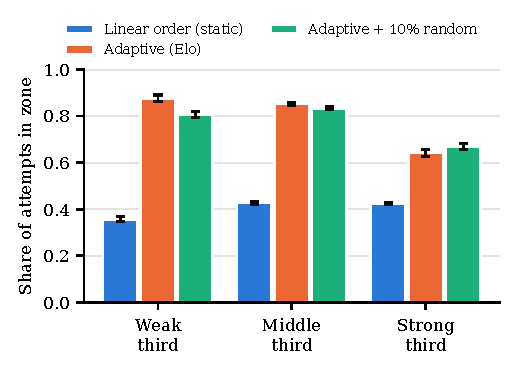
\includegraphics[width=\columnwidth]{figures/zone_by_tercile.pdf}
\caption{Share of attempts in the zone of attainable difficulty by ability tercile (mean and 95\% CI, 1,500 simulated students per policy).}
\label{fig:zone}
\end{figure}

\textit{RQ3.} The update step strongly affected the ability estimate (ANOVA $F(3, 16) = 2287$, $\eta^2 = 0.998$); $K = 0.2$ gave the lowest RMSE of 0.44 logits (Fig.~\ref{fig:rmse}). Under purely adaptive selection, all predictions are close to 0.7 and AUC is uninformative (0.54--0.57 for both models). On the randomly assigned 10\% of tasks, the Elo prediction reached an AUC of 0.807 versus 0.781 for static labels (difference 0.026, 95\% CI 0.014--0.038).

\begin{figure}[t]
\centering
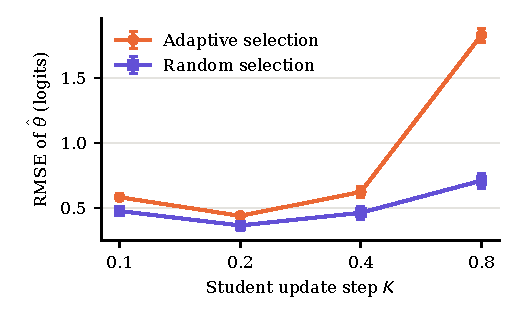
\includegraphics[width=\columnwidth]{figures/rmse_by_k.pdf}
\caption{Error of the ability estimate versus the Elo update step $K$ (mean and 95\% CI over 5 runs).}
\label{fig:rmse}
\end{figure}

\textit{Robustness and cold start.} Because the simulated students follow the same logistic model as the Elo rating, we repeated the study with a misspecified generator: a guessing rate of 0.1, a slip rate of 0.1, and ability growing by 0.02 logits after each success. Adaptive selection still kept more attempts in the zone than the linear order (0.88 vs.\ 0.66, $d = 1.3$), but the advantage of Elo over static labels shrank to 0.014 AUC (95\% CI 0.007--0.022). In a second variant the initial estimate $\hat\theta$ was taken from a noisy pre-test ($\theta^{*}$ plus $\mathcal{N}(0, 0.5)$ noise). This raised the zone share of the strong third from 0.64 to 0.81 and cut overly easy tasks in their first 15 attempts from 0.76 to 0.27 (Table~\ref{tab:robust}).

\begin{table}[t]
\caption{Robustness checks for the adaptive policy (mean of 5 runs)}
\label{tab:robust}
\centering
\begin{tabular}{@{}lccc@{}}
\toprule
Metric & Base & Misspecified & Pre-test start \\
\midrule
Zone share, adaptive & 0.79 & 0.88 & 0.89 \\
Zone share, linear & 0.40 & 0.66 & 0.40 \\
Zone share, strong third & 0.64 & 0.74 & 0.81 \\
Too easy, strong, first 15 & 0.76 & 0.59 & 0.27 \\
AUC gain of Elo (mixed) & 0.026 & 0.014 & 0.039 \\
\bottomrule
\end{tabular}
\end{table}

\textit{System cost.} The whole model takes under 10~$\mu$s per event. With Redis storage the service sustained about 1,700 requests per second at 64 concurrent clients with a p95 latency of 53~ms, well below the 100~ms target.

\section{Discussion}
The results support the mechanism behind adaptive gamification: matching difficulty to the student roughly doubles the share of attainable tasks, and the benefit concentrates on weaker students. If the mechanism carries over to real learners, the difference in engagement between adaptive and static gamification should be largest in the lowest pre-test tercile. This offers one explanation for the small average effects in~\cite{sailer2020}: a benefit concentrated in part of the class is diluted by averaging.

The cold-start problem is a practical risk because the first week of a course is when engagement forms. Initialising $\hat\theta$ from the pre-test, which the experimental design already includes, removes most of the problem in simulation; a decreasing update step as proposed in~\cite{pelanek2016} is an alternative when no pre-test is available. For RQ3, the advantage of Elo over static labels is small; assigning 10\% of tasks at random costs 2 percentage points of success rate and makes the comparison valid.

\textit{Limitations.} The base simulation follows the same logistic model as the Elo rating. The misspecified variant shows that the selection result holds but the AUC advantage of Elo roughly halves, so RQ3 should be treated as a check of model quality rather than a main finding. The zone bounds 0.5--0.85 are a modelling choice; the bound-free mean distance $|P - p^{*}|$ in Table~\ref{tab:policies} leads to the same conclusion. The simulation contains no fatigue, learning during the course, cheating or dropout, and it says nothing about engagement itself.

\textit{Experimental protocol.} The model will be tested in a randomised between-subjects experiment with three conditions: no game layer, static gamification and adaptive gamification. Students will practise for four weeks after a pre-test; outcomes are an engagement index computed from event logs, the share of solved tasks, normalised learning gain and retention two weeks later. The analysis plan (ANCOVA with the pre-test as covariate, Holm correction, effect sizes with confidence intervals) will be preregistered before data collection, and participation requires informed consent and approval of the university ethics committee.

\section{Conclusion}
An Elo-based model can keep programming tasks within reach for most students, at negligible computational cost, and it helps weaker students most. Its main weakness, a slow start for strong students, has known remedies. Whether these properties translate into higher engagement and learning will be answered by the controlled experiment described above.

\section*{Data Availability}
Code, simulation scripts, raw results and figures are available at~\cite{nirm2026code} under the Apache-2.0 license. All results in this paper are reproduced with \texttt{make policies} and \texttt{make analyze}.

\bibliographystyle{IEEEtran}
\bibliography{references}

\end{document}
